\qrchapter{https://forgottenpillar.com/rsc/sw-fp-chapter21}{Kukumbuka mwanzo} \label{chap:remembering-the-beginning}

\egw{\textbf{Hatuwezi wakati wowote ule kuwa na \underline{upotoshaji} wowote juu ya haya masomo laini na muhimu ya ukweli ambayo yamekuwa imani ya watu wetu tangu 1844.}}[Lt300-1903.9; 1903][https://egwwritings.org/read?panels=p7705.15]

Maana ya kweli ya \emcap{Kanuni za Msingi} ni mtazamo mpana zaidi wa ujumbe wa wale malaika watatu.

\egw{\textbf{Sisi ni watu wa Mungu wanaozishika amri}. Kwa miaka hamsini iliyopita kila awamu ya uzushi umeletwa juu yetu, ili \textbf{kuziba akili zetu kuhusu mafundisho ya neno,—\underline{hasa kuhusu huduma ya Kristo mbinguni patakatifu}, na ujumbe wa mbinguni kwa siku hizi za mwisho, kama \underline{ulivyotolewa na malaika wa sura ya kumi na nne ya Ufunuo}}. Ujumbe wa kila namna na aina umehimizwa dhidi ya Waadventista Wasabato, \textbf{kuchukua nafasi ya ile kweli ambayo}, \textbf{hatua kwa hatua}, imetafutwa kwa kujifunza kwa maombi, na kushuhudiwa kwa uwezo wa kutenda miujiza wa Bwana. \textbf{Lakini alama za njia ambazo zimetufanya tulivyo, zinapaswa kuhifadhiwa, na itahifadhiwa}, kama vile Mungu ameonyesha kupitia neno Lake na ushuhuda wa Roho wake. \textbf{Yeye Anatutaka kushikilia kwa uthabiti, kwa mshiko wa imani, \underline{kanuni za msingi} ambazo zinatokana na mamlaka isiyotiliwa shaka}.}[SpTB02 59.1; 1904][https://egwwritings.org/read?panels=p417.299]

Hapa tunaona jinsi Ellen White alivyoelezea ujumbe wa \emcap{Kanuni za Msingi} kama ujumbe wa wale malaika watatu’, kutoka sura ya kumi na nne ya Ufunuo, na kama ujumbe kuhusu huduma ya Kristo katika patakatifu pa mbinguni. Hoja ya kwanza ya \emcap{Kanuni za Msingi}, ambazo zimejadiliwa sana hapa, zinajibu swali muhimu linalotolewa na malaika wa kwanza katika sura ya kumi na nne ya Ufunuo: \textit{Mungu yupi tunayepaswa kumwabudu}?

\bible{Mcheni \textbf{Mungu}, na \textbf{kumtukuza \underline{yeye}}; kwa maana \textbf{saa ya hukumu \underline{yake} imekuja}: \textbf{mwabudu \underline{yeye}} aliyezifanya mbingu, na nchi, na bahari, na chem-chemi za maji.}[Ufunuo 14:7]

Ni Mungu Yupi tunayepaswa kumwabudu, aliyetangazwa na malaika wa kwanza? Katika wigo wa wakati sisi tunapata majibu tofauti kwa swali hili. Leo jibu ni Mungu aliye tatu, au Mungu wa Utatu, kama ilivyotolewa katika Imani za Msingi za Waadventista Wasabato. Lakini, tunauliza swali: Je! ni Mungu gani ambaye waanzilishi wa Kiadventista walimwabudu? Ujumbe wa malaika wa kwanza umejumuishwa kwa wakati wa kinabii, ambao ulitimizwa katika nyakati za waanzilishi wetu. Kusudi lote nyuma ya kazi yao ilikuwa ni tangazo la jumbe za malaika watatu. Mnamo 1844, saa ya hukumu ya Mungu ilikuwa imekuja. Ikiwa Mungu wa Utatu ndiye Mungu ambaye saa yake ilikuwa imefika, na waanzilishi wetu hawakuabudu Utatu, je, hawakushindwa katika kusudi lao la kuunda harakati hii?

Hebu tuchunguze historia ya harakati zetu za kinabii kwa swali hili: je waanzilishi wetu walimwabudu Mungu wa kweli katika kutangaza ujumbe wa malaika wa kwanza? Tunasoma maelezo ya matukio ya 1844.

\egw{\textbf{Kama wanafunzi wa kwanza, William Miller na washirika wake hawakuelewa wao wenyewe, ufahamu wa kikamilifu na umuhimu wa ujumbe waliobeba}. Makosa ambayo yalikuwa yamekita mizizi kwa muda mrefu yaliwazuia kufikia kwenye tafsiri sahihi ya jambo muhimu katika unabii. Kwa hiyo, ingawa walitangaza ujumbe wa Mungu ulioka-bidhiwa kwao kutolewa kwa ulimwengu, kutouelewa maana yake kuli-wafanya kukatishwa tamaa.}[GC 351.2; 1888][https://egwwritings.org/read?panels=p132.1604]

\egwnogap{Katika kueleza Danieli 8:14, ‘Hata \textbf{siku elfu mbili na mia tatu; basi itakuwa \underline{patakatifu pasafishwe}},’ Miller, kama ilivyosemwa, alikubali maoni aliyopokea kwa ujumla kwamba dunia ni patakatifu, na aliamini kwamba utakaso wa patakatifu uliwakilisha utakaso wa dunia kwa moto wakati wa kuja kwake Bwana. Kwa hiyo, aligundua kwamba mwisho wa siku 2300 ulikuwa umetabiriwa kwa hakika, alihitimisha kwamba huu uli-funua wakati wa ujio wa pili. Kosa lake lilitokana na kukubali maoni ya watu wengi kuhusu mahali patakatifu pa patakatifu.}[GC 352.1; 1888][https://egwwritings.org/read?panels=p132.1607]

\egwnogap{Katika mfumo wa mfano, ambao ulikuwa ni kivuli cha dhabihu na \textbf{ukuhani wa Kristo}, \textbf{utakaso wa patakatifu ulikuwa huduma ya mwisho kufanywa na kuhani mkuu }katika kila mwaka wa wizara.\textbf{ Ilikuwa ni kazi ya kufunga ya upatanisho—kuondolewa au kuondoa dhambi kutoka kwa Waisraeli}. \textbf{Ilitanguliza kazi ya kufunga katika wizara ya Kuhani wetu Mkuu mbinguni, katika kuondolewa au kufuta dhambi za watu wake, ambazo zimesajiliwa katika kumbukumbu za mbinguni}. \textbf{Huduma hii inahusisha kazi ya \underline{uchunguzi, kazi ya hukumu}; na mara moja hutanguliza kuja kwa Kristo} ndani ya mawingu ya mbinguni kwa nguvu na utukufu mkuu; kwa maana ajapo, kila kesi itakuwa imeamuliwa. Yesu asema hivi: ‘Ujira wangu u pamoja nami, kumlipa kila mtu kadiri ya kazi yake.’ Ufunuo 22:12. \textbf{Ni kazi hii ya hukumu, mara moja inayotangulia ujio wake wa pili, unaotangazwa katika \underline{ujumbe wa malaika wa kwanza wa Ufunuo 14:7}: ‘Mcheni \underline{Mungu}, na kumtukuza; \underline{kwa maana saa ya hukumu yake imekuja}.}’}[GC 352.2; 1888][https://egwwritings.org/read?panels=p132.1608]

\egwnogap{\textbf{Wale waliotangaza onyo hili walitoa ujumbe ufaao kwa wakati ufaao}. Lakini kama wanafunzi wa kwanza walitangaza, 'Wakati umetimia, na ufalme wa Mungu umekaribia,' msingi juu ya unabii wa Danieli 9, huku wakishindwa kutambua kwamba kifo cha Masihi kilikuwa kimetabiriwa katika andiko hilohilo, \textbf{kwa hiyo Miller na washirika wake walihubiri ujumbe huo kwa msingi kwenye \underline{Danieli 8:14 na Ufunuo 14:7}, na kushindwa kuona kwamba bado kulikuwa na jumbe nyingine zilizoletwa katika Ufunuo 14}, ambazo pia zilipaswa kutolewa kabla ya ujio wa Bwana. Kama vile wanafunzi walikosea kuhusiana na ufalme ambao ungesimamishwa mwisho wa majuma sabini, hivyo Waadventista walikosea kuhusiana na tukio la kutendekeka kwa kumalizika kwa siku 2300. Katika visa vyote viwili kulikuwa na kukubaliana au tuseme ufuasi kwa, makosa maarufu ambayo yalipofusha akili kwa ukweli. Madarasa yote mawili yalitimiza mapenzi ya Mungu katika kufikisha ujumbe ambao alitamani upewe, na wote wawili, kupitia kwa kutoelewa kwao ujumbe wao, walihisi uchungu wa kukata tamaa.}[GC 352.3; 1888][https://egwwritings.org/read?panels=p132.1609]

\begin{figure}[hp]
    \centering
    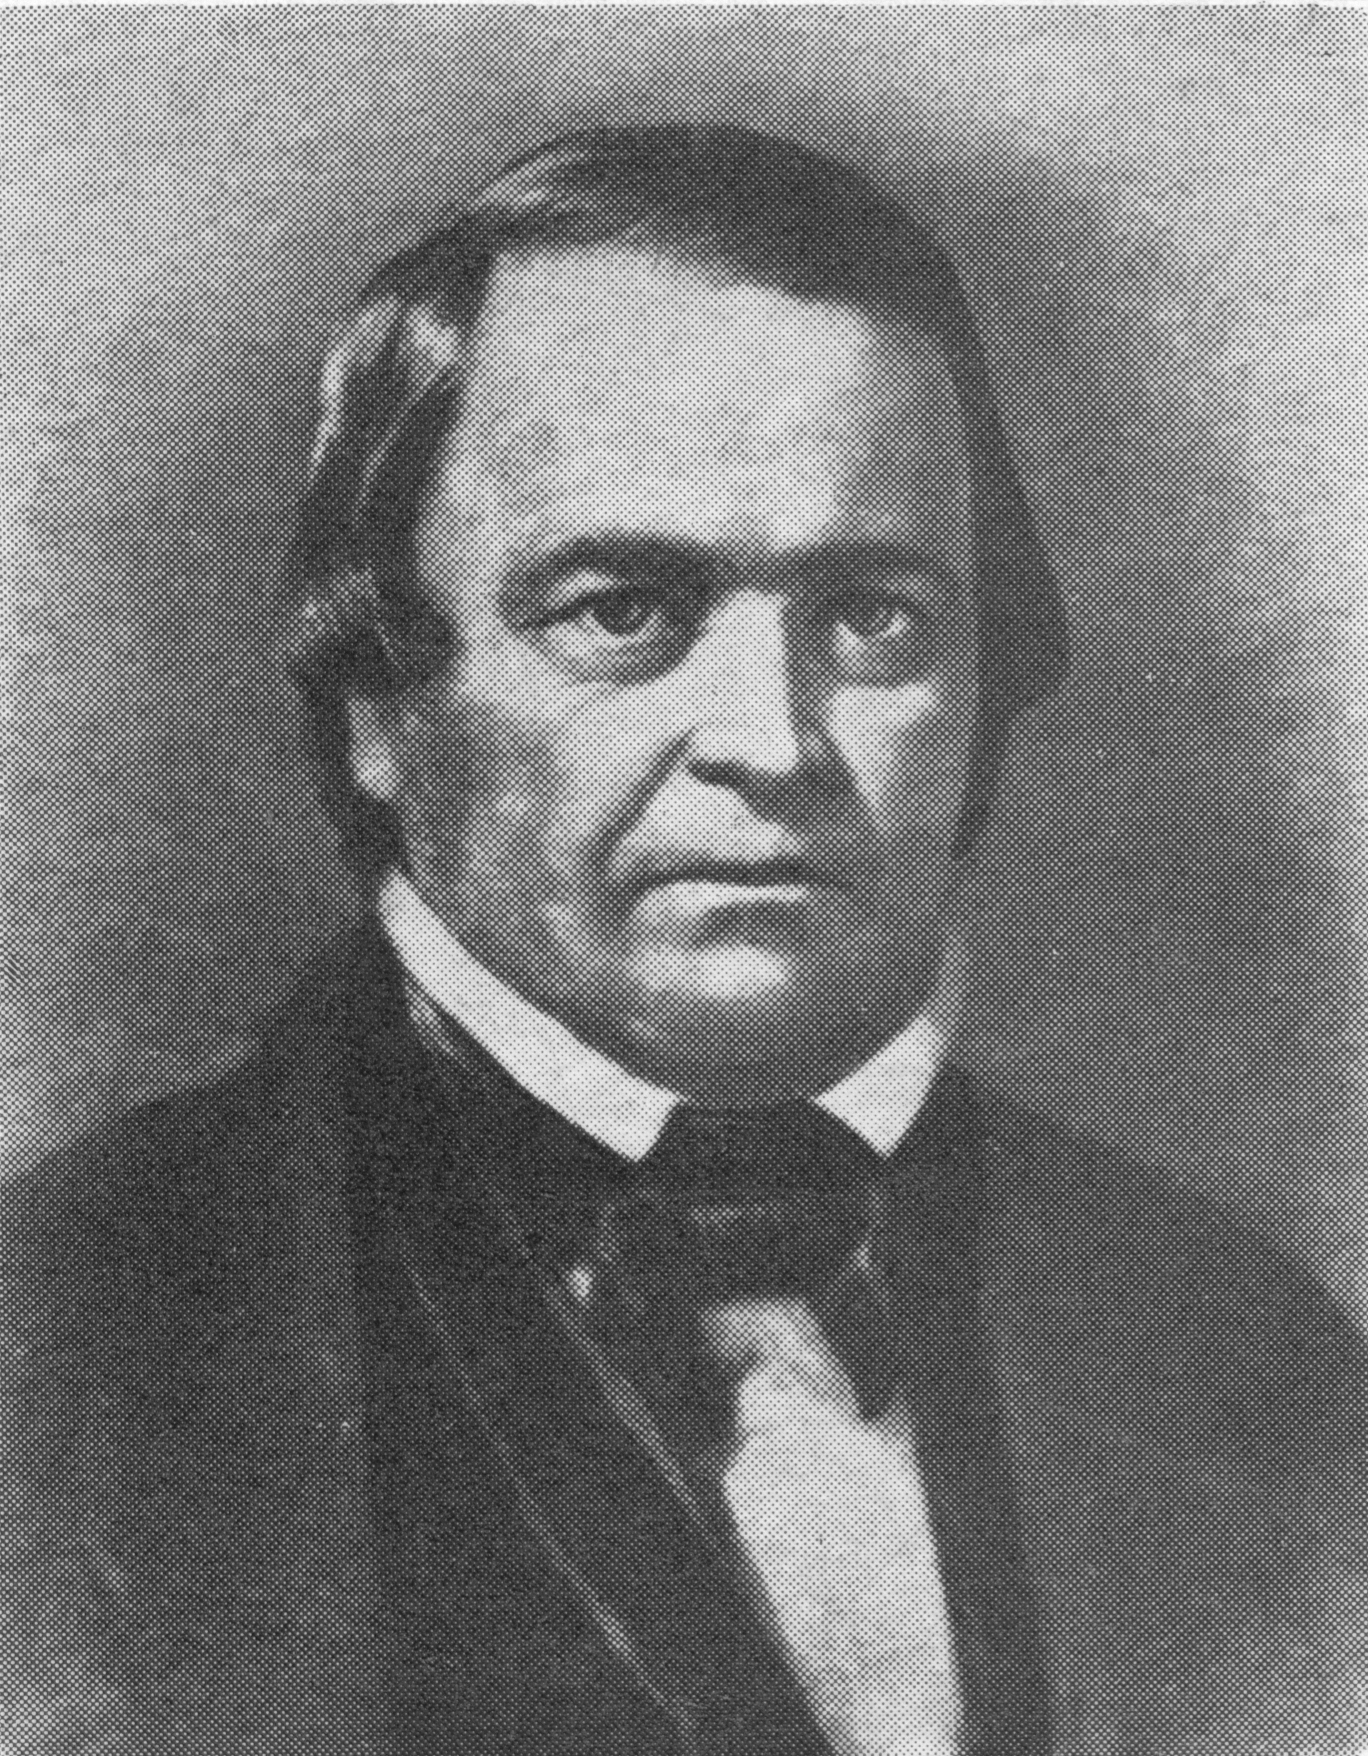
\includegraphics[width=1\linewidth]{images/william-miller.jpg}
    \caption*{William Miller (1782-1849)}
    \label{fig:w-miller}
\end{figure}

Katika kusoma maelezo ya kukata tamaa kubwa, uliona jibu la swali, "\textit{Mungu ambaye hukumu yake imekuja ni nani?}" Ujumbe wa malaika wa kwanza kutoka Ufunuo 14:7 inapatana sawasawa na wakati wa kinabii unaotangazwa katika Danieli 8:14. Hukumu ambayo imekuja ilikuwa ni hukumu ya uchunguzi, iliyoanza mwaka 1844. Biblia kwa uwazi inaeleza ambaye saa ya hukumu imekuja katika ujumbe wa malaika wa kwanza. Wacha tuisome ndani Biblia na uone maoni ya Ellen White.

\egw{‘Nikaona,’ asema nabii Danieli, \textbf{‘mpaka viti vya enzi vikawekwa, na Mmoja aliyekuwa \underline{wa Kale wa Siku} \underline{ameketi}}: \textbf{mavazi yake} yalikuwa meupe kama theluji, na \textbf{nywele za kichwa chake} kama sufu safi; \textbf{Kiti chake cha enzi kilikuwa miali ya moto}, na magurudumu yake ni moto uwakao. Mto wa moto ulitolewa na ukatoka mbele zake; maelfu elfu wakamtumikia, na elfu kumi mara elfu kumi wakasimama mbele zake: \textbf{\underline{hukumu ikawekwa, na vitabu vikafunguliwa}}.’ Danieli 7:9, 10, R.V.}[GC 479.1; 1888][https://egwwritings.org/read?panels=p132.2169]

\egwnogap{\textbf{Hivyo ndivyo ilivyoonyeshwa kwenye maono ya nabii ile siku kuu na adhimu wakati wahusika na maisha ya watu yatapitishwa mbele ya Hakimu wa Dunia yote, na kila mtu atapewa ‘kulingana na kazi zake.’ \underline{Mzee wa Siku ni Mungu Baba}.} Mtunga-zaburi asema hivi: \textbf{‘Kabla }haijazaliwa milima, au wewe kuumba dunia na ulimwengu, \textbf{Tangu milele hata milele}, \textbf{Wewe ndiwe Mungu}.’ Zaburi 90:2. \textbf{\underline{Yeye ndiye chanzo cha viumbe vyote, na chemchemi ya sheria zote ambaye Anayesimamia hukumu}}. Na malaika watakatifu kama watumishi na mashahidi, kwa idadi ‘elfu kumi mara elfu kumi, na maelfu ya maelfu,’ huhudhuria mahakama hii kubwa.}[GC 479.2; 1888][https://egwwritings.org/read?panels=p132.2170]

\egwnogap{\textbf{‘Na tazama, mmoja aliye kama \underline{Mwana wa Adamu} akaja pamoja na mawingu ya mbinguni, akaja kwa \underline{Mzee wa Siku}, nao \underline{wakamleta karibu naye}}. Naye akapewa mamlaka, na utukufu, na ufalme, ili watu wote, na mataifa, na lugha, wamtumikie Yeye: mamlaka yake ni mamlaka ya milele, ambayo hayatapita kamwe.’ Danieli 7:13, 14. \textbf{Kuja kwa Kristo kumeelezwa hapa si kuja kwake mara ya pili duniani}. \textbf{\underline{Anakuja kwa Mzee wa Siku mbinguni} ili kupokea mamlaka na utukufu na ufalme}, \textbf{ambao atapewa mwisho wa kazi yake kama mpatanishi}. \textbf{\underline{Ni kuja huku, na si ujio wake wa pili kwa dunia, ambao ulitabiriwa katika unabii kwamba ungetukia siku ya kumalizika kwa siku 2300 katika 1844}}. \textbf{Kuhudhuriwa na malaika wa mbinguni, kuhani wetu Mkuu anaingia patakatifu pa patakatifu na anaonekana katika \underline{uwepo wa Mungu}} akijishughulisha na matendo ya mwisho ya huduma Yake kwa niaba ya mwanadamu—\textbf{kufanya kazi ya uchunguzi hukumu} na \textbf{kufanya upatanisho} kwa wote ambao wameonyeshwa kustahiki faida zake.}[GC 479.3; 1888][https://egwwritings.org/read?panels=p132.2171]

Jibu ni rahisi na la moja kwa moja: Mungu wa waanzilishi wetu alikuwa Mzee wa Siku. \egwinline{Mzee wa Siku ni Mungu Baba}. Yeye ndiye \textit{nafsi wa kibinafsi}, \textit{wa kiroho}. Tunaona hii ndani ya Maelezo kwake: \bible{Ambaye vazi lake lilikuwa jeupe kama theluji, na nywele za kichwa chake kama sufu safi: kiti chake cha enzi kilikuwa kama mwali wa moto, na magurudumu yake kama moto uwakao.}[Danieli 7:9]. Katika kumalizika kwa unabii wa siku 2300, katika 1844, \bible{Saa ya hukumu yake imekuja}[Ufunuo 14:7], \bible{Mzee wa siku aliketi} na \bible{hukumu ikawekwa, na vitabu kufunguliwa.}[Danieli 7:9,10]. Mungu kutoka kwa ujumbe wa malaika wa kwanza ni Mzee wa Siku. Mapainia hawakuwa wajinga kuhusu ukweli kumhusu Mungu. Waliamini \others{Kwamba kuna \textbf{Mungu Mmoja}, \textbf{\underline{huluki wa kibinafsi, wa kiroho}}, \textbf{muumba wa vitu vyote}, muweza wa yote, mjuzi wa yote, na WA milele, asiye na kikomo katika hekima, utakatifu, haki, wema, ukweli, na rehema; asiyebadilika, na \textbf{\underline{Yuko kila mahali kupitia kwa mwakilishi wake, Roho Mtakatifu}}. Zab. 139:7.}[First point of the Fundamental Principles.] Huyu ndiye Mungu mmoja Baba, Mzee wa Siku, \others{muumba wa vitu vyote}, nasi tunapaswa \bible{kumuabudu yeye ambaye aliyeziumba mbingu, na nchi, na bahari, na chemchemi za maji}[Ufunuo 14:7]. Yeye \bible{aliumba vitu vyote katika Yesu Kristo}[Waefeso 3:9].

Leo, ujumbe wa malaika wa kwanza haujapoteza umuhimu wake. Ujumbe wa malaika wa pili na wa tatu unategemea ujumbe wa kwanza na ujumbe wa kwanza unahitaji tu hatua kwa upande wetu. Tunapaswa kumwabudu Mungu. Hasa zaidi, tunapaswa kuabudu Mungu wa kweli. Katika pambano la mwisho na la kuhitimisha, kutakuwa na aina mbili za waabudu, kama tulivyoambiwa katika Ufunuo 13 na 14.

\bible{Na wote wakaao juu ya nchi watamsujudu \normaltext{[yule mnyama]}, \textbf{ambao majina yao hayajaandikwa katika kitabu cha uzima cha Mwana-Kondoo} aliyechinjwa tangu kuwekwa misingi ya ulimwengu.}[Ufunuo 13:8]

Kundi linalomwabudu mnyama litapokea alama ya mnyama. Dunia nzima italazimishwa kumwabudu yule mnyama na sanamu yake kwa tisho la kifo.

\bible{Naye \normaltext{[mnyama]} alikuwa na uwezo wa kuipa uhai \textbf{sanamu ya yule mnyama}, ili sanamu ya mnyama inene na kuwafanya \textbf{watu wote wasioiabudu sanamu ya mnyama lazima wauawe}.}[Ufunuo 13:15]

Hatupaswi kushiriki katika ibada hii. Hebu tujifunze na kuwa na imani kama wale marafiki watatu wa Danieli waliokataa kuabudu sanamu ya Mfalme Nebukadneza. Mnyama aliwakilishwa katika Ufunuo 13, ambaye hunyang'anya watu dhamira zao kwa kuhatarisha maisha yao, ni upapa. Rafiki mpendwa, usidanganywe. Mungu wa Papa ni Mungu wa Utatu. Usipuuze hilo.

Tunapaswa kumwabudu Mzee wa Siku kama inavyotangazwa katika ujumbe wa malaika wa kwanza. Huyu ni Mungu Muumba aliyeumba kila kitu kupitia Mwanawe, Yesu Kristo. Huyu ni Mungu kutoka hoja ya kwanza ya \emcap{Kanuni za Msingi}. Waanzilishi wetu walipata hili vizuri.

Uelewa wa kweli wa utume na madhumuni ya harakati ya Waadventista Wasabato yapaswa kuwa uthibitisho kamili kwamba fundisho la Utatu ni fundisho geni kwetu. Tumepata kuishia hapa tulipo leo kwa sababu tumesahau \egwinline{\textbf{njia aliyotuongoza Bwana, na \underline{mafundisho Yake} katika historia yetu iliyopita.}}[LS 196.2; 1915][https://egwwritings.org/read?panels=p41.1083] Inasikitisha sana kuona jinsi wataalamu wetu wa Kiadventista wanadai kwamba waanzilishi wetu hawakuelewa kwa usahihi fundisho la Mungu. Ingekuwa hivyo kweli, mapainia wetu wangekosa kutangaza ujumbe wa malaika wa kwanza. Hawakushindwa. Tumeshindwa.

\others{\textbf{Wengi wa waanzilishi wa Waadventista Wasabato hawangeweza kujiunga na kanisa leo ikiwa walipaswa kujiunga na Imani za Msingi za dhehebu}.}\others{\textbf{Hasa zaidi, wengi hawataweza kukubaliana na imani nambari 2, ambayo inahusika pamoja na fundisho la Utatu.} Kwa Joseph Bates Utatu lilikuwa fundisho lisilo la kimaandiko, kwa James White ulikuwa ni ule “upuuzi wa zamani wa Utatu,” na kwa M. E. Cornell ulikuwa tunda la ukengeufu mkuu, pamoja na mafundisho ya uwongo kama vile kushika Jumapili na kutokufa kwa nafsi.}[George Night, Ministry Magazine, October 1993][https://www.ministrymagazine.org/archive/1993/10/adventists-and-change]

Fundisho la Utatu ni fundisho linalodhoofisha msingi wa imani yetu, msingi ambao uliwekwa mwanzoni mwa kazi yetu. Tofauti kati ya ukweli na makosa iko katika hermeneutiki—njia ya kutafsiri Biblia. Hebu tuchunguze kwa kina suala hili.

\begin{titledpoem}
\stanza{
    In faith's first light, they sought His face, \\
    A vision pure, of divine grace. \\
    The pioneers, with vision clear, \\
    In 1844, held God so dear.
}

\stanza{    
    "The hour of judgment has come," they cried, \\
    To a world, both far and wide. \\
    The Ancient of Days, they did proclaim, \\
    Not a trinity, but a singular name.
}

\stanza{    
    Ellen White, with pen in hand, \\
    Spoke of a sanctuary, not of earthly land. \\
    A message of heaven, pure and bright, \\
    Guiding the faithful through the night.
}

\stanza{    
    The first angel’s message, a call to revere, \\
    God the Father, whom we should fear. \\
    "Who is the God we are to adore?" \\
    Not a trinity—this, they implored.
}

\stanza{    
    The Trinity, a concept unembraced, \\
    By pioneers, who in God's word traced. \\
    The Father, the Ancient, they did declare, \\
    His judgment and mercy, beyond compare.
}

\stanza{
    Yet, whispers now, through time have spread, \\ 
    A trinity's shadow, causing dread. \\
    If this be the God they were to declare, \\
    Their mission failed, caught in despair.
}

\stanza{
    But this is a falsehood, bold and cold, \\
    A narrative modern, but wrongly told. \\
    The Father they worshiped, with fervent zeal, \\
    Was the true God, their mission real.
}

\stanza{
    In unity, may we seek His face, \\
    Embracing truth, with grace and grace. \\
    The pioneers' vision, let us not lose, \\
    For in their footsteps, we must choose.
}

\stanza{
    To worship the God, of days of old, \\
    The Ancient of Days, as was foretold. \\
    In Revelation’s message, clear and bright, \\
    Guiding us still, through darkest night.
}
\end{titledpoem}